\begin{frame}{Le livre hypermédiatique}
    \begin{columns}[T,onlytextwidth]
        \column{0.50\linewidth}
        \small
        \begin{itemize}
            \item Créé par et pour le numérique, et non en complément ou par imitation d’un « original papier ».\\
            \item  \href{http://revuebleuorange.org/oeuvre/08/livres-dartistes-livres-numeriques-manifeste}{Manifeste de la revue bleu orange} paru en 2015

        \end{itemize}

        \column{0.50\linewidth}
        \centering
        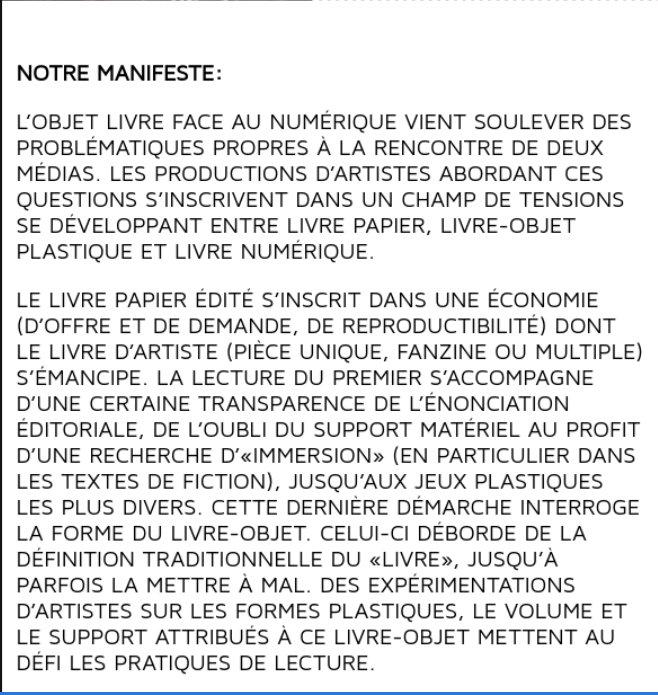
\includegraphics[width=.90\columnwidth]{Images/revue_bleuorange_manifeste.png}
    \end{columns}
\end{frame}

\begin{frame}{Le livre hypermédiatique}
    \centering
    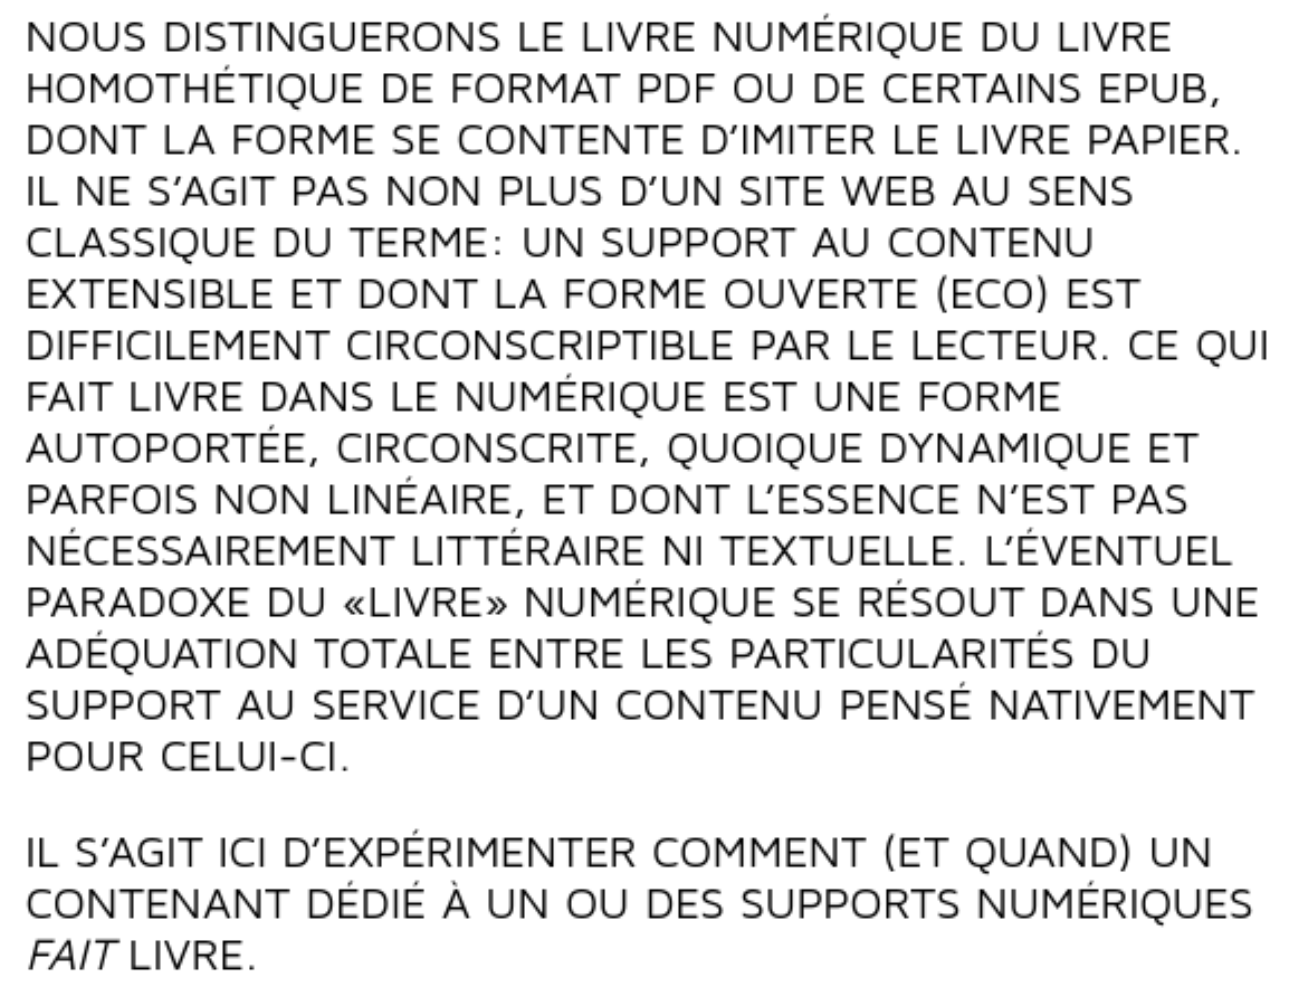
\includegraphics[width=.60\textwidth]{Images/suite_manifeste.png}
\end{frame}

\begin{frame}{le livre-application}
    Dépend de l'installation et compatibilité d'un outil: problème de pérennité, entretien de l'appli et du code.\\
    \textbf{Exemple:}
    \begin{itemize}
        \item \href{https://vimeo.com/74614087?fl=pl&fe=cm}{Conduit d'aération}: récit pour Ipad puis epub3.
        \item Enterre-moi mon amour (2017)
    \end{itemize}
\end{frame}